\documentclass{standalone}
\usepackage{tikz}
\usetikzlibrary{automata} % Import library for drawing automata
\usetikzlibrary{positioning} % ...positioning nodes
\usetikzlibrary{arrows}
\begin{document}
    
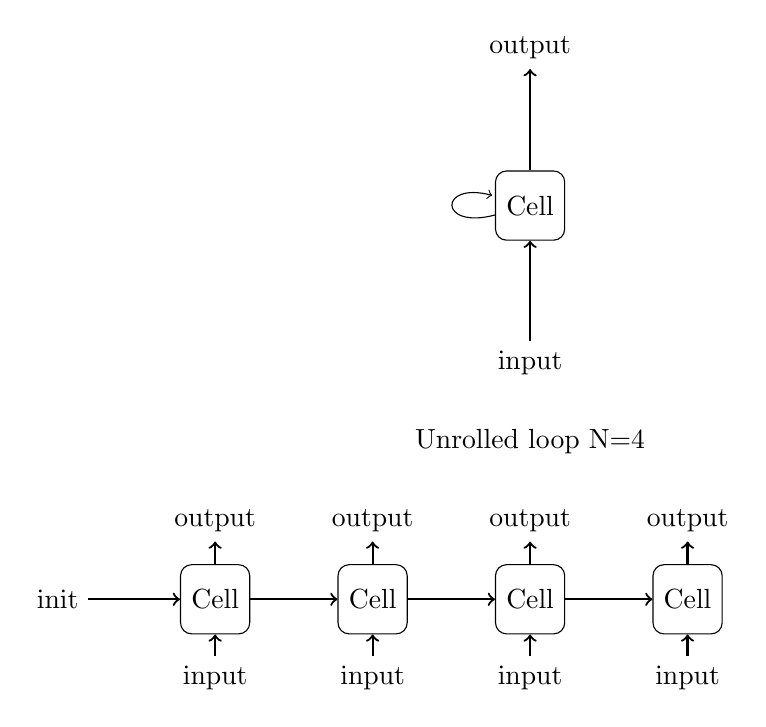
\begin{tikzpicture}
\tikzset{every state/.append style={rectangle, rounded corners}}
\path (0,0) node(o) {output};
\path (0,0-4) node(i) {input};

\node[state] (q1) at(0,-2) {Cell};
\draw (q1) edge [loop left ] (q1);
\draw (q1) edge[->,thick]  (o);
\draw (i) edge[->,thick]  (q1);
\foreach \x in {-4,-2,0,2} {
\node[state] (\x) at (\x,-7) {Cell};
\path (\x,-6) node(o) {output};
\path (\x,-8) node(i) {input};
\path (\x) edge[->,thick] (o);
\path (i) edge[->,thick] (\x);
}
\path (0,-5) node {Unrolled loop N=4};
\draw (-4) edge[->,thick] (-2);
\draw (-2) edge[->,thick] (0);
\draw (0) edge[->,thick] (2);

\path (-6,-7) node (init) {init};
\draw (init) edge[->,thick] (-4);

\end{tikzpicture}
\end{document}
